\chapter{Eléments d’histoire de la présence musulmane en France}
\mn{LUNDI 8 NOVEMBRE 2021 (1
er cours)}

Eléments d’histoire de la présence musulmane en France : Moyen-Age, soldats
nord-africains (période coloniale), Grande mosquée de Paris, et immigration de
travail.

% -------------------------------------------------------------------
\section{Premiers contacts (Moyen-Âge, Septimanie, Fraxinet, Moussais/Poitiers…)}



\paragraph{Les incursions dans le Sud de la France (Septimanie/Narbonne) – 719-759}


\paragraph{Le « Massif des maures » (Fraxinet) entre 850 et 973}
 
 Fraxinet ou Fraxinetum est un établissement pirate puis comptoir  sarrasin du xe siècle dans le golfe de Saint-Tropez, dans le Var. Le territoire de la cité, aux limites mal définies (peut-être la commune actuelle de La Garde-Freinet), est conquis par des marins venus d'Al-Andalus vers 890 et repris par le comte de Provence Guillaume Ier (surnommé ensuite « le Libérateur ») en 973 après la bataille de Tourtour.
 
 \begin{marginfigure}
    \centering
    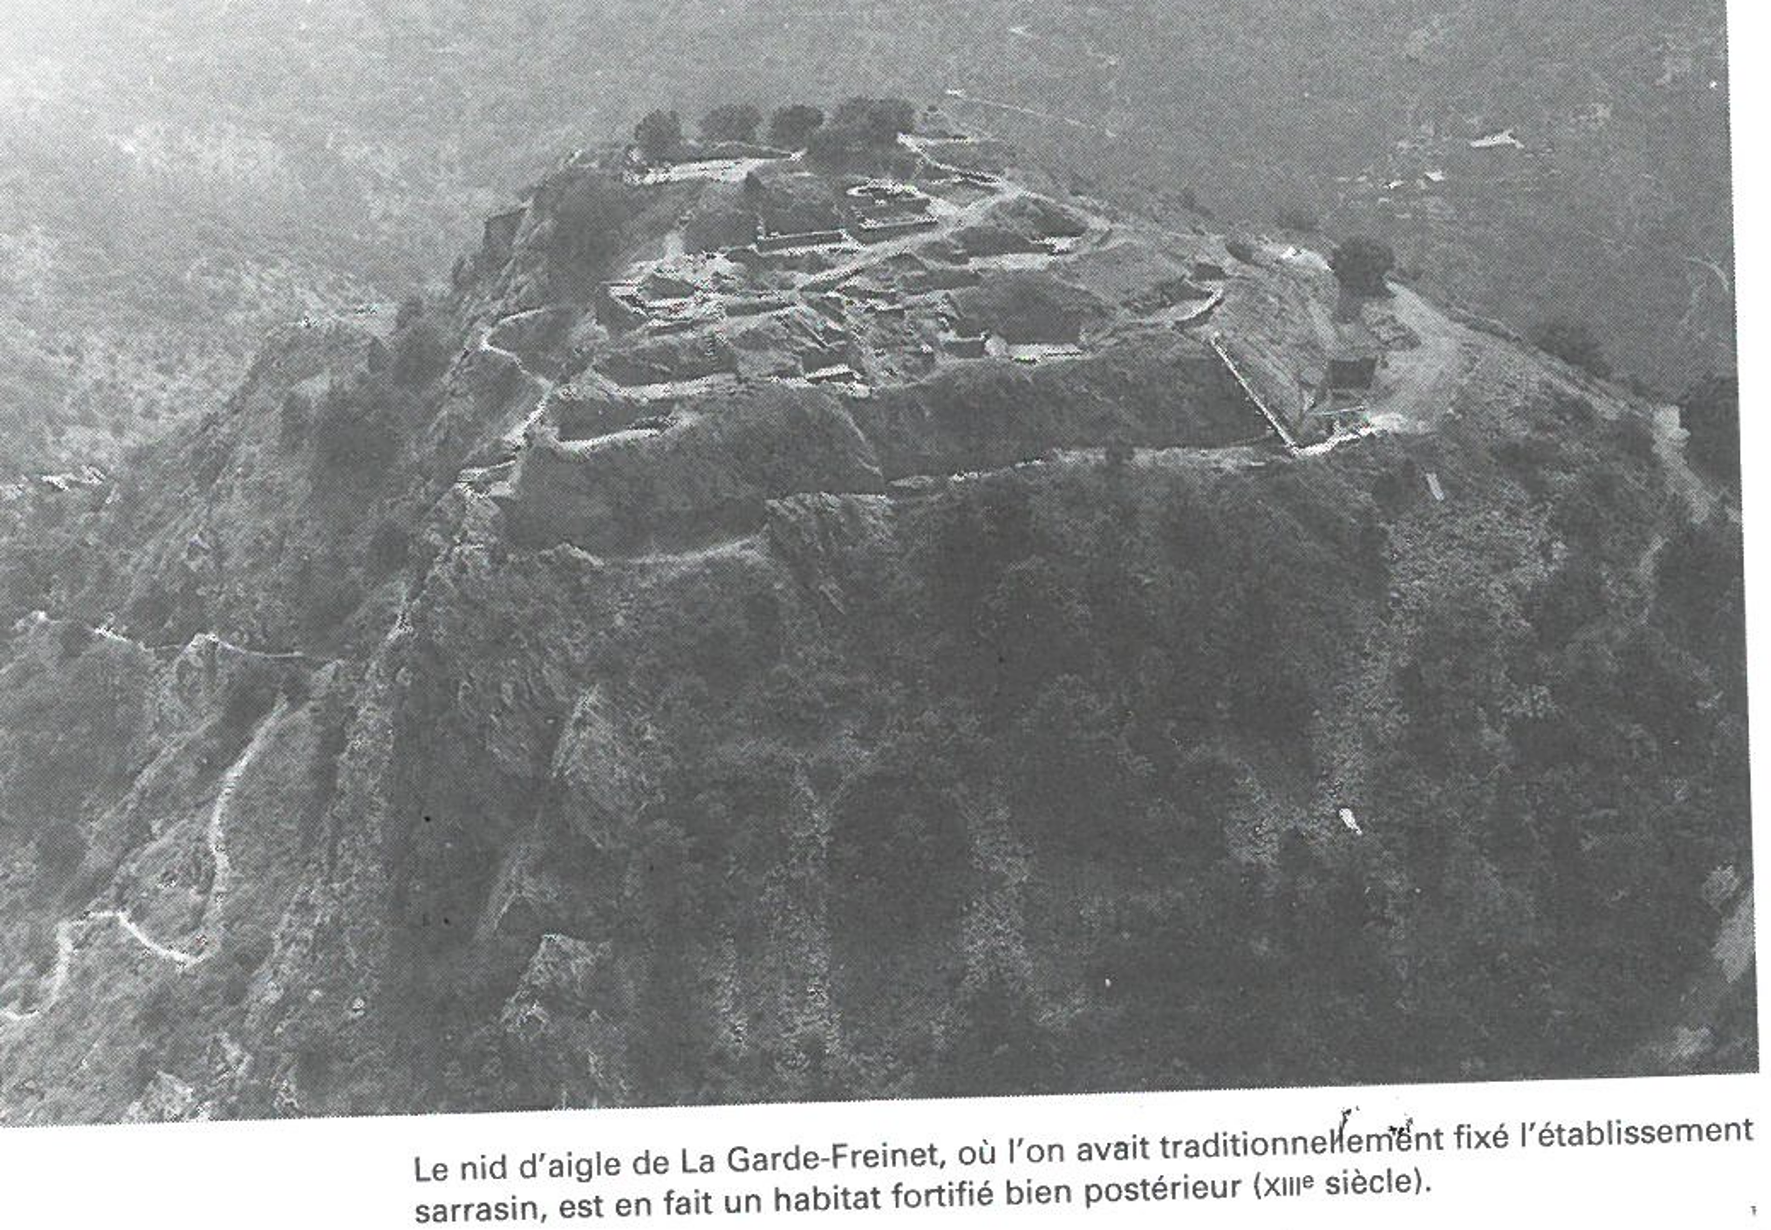
\includegraphics[width=\textwidth]{Images/nidAigle.png}
    \caption{Le nid d'aigle}
    \label{fig:nidAigle}
\end{marginfigure}

\begin{figure}[h!]
    \centering
    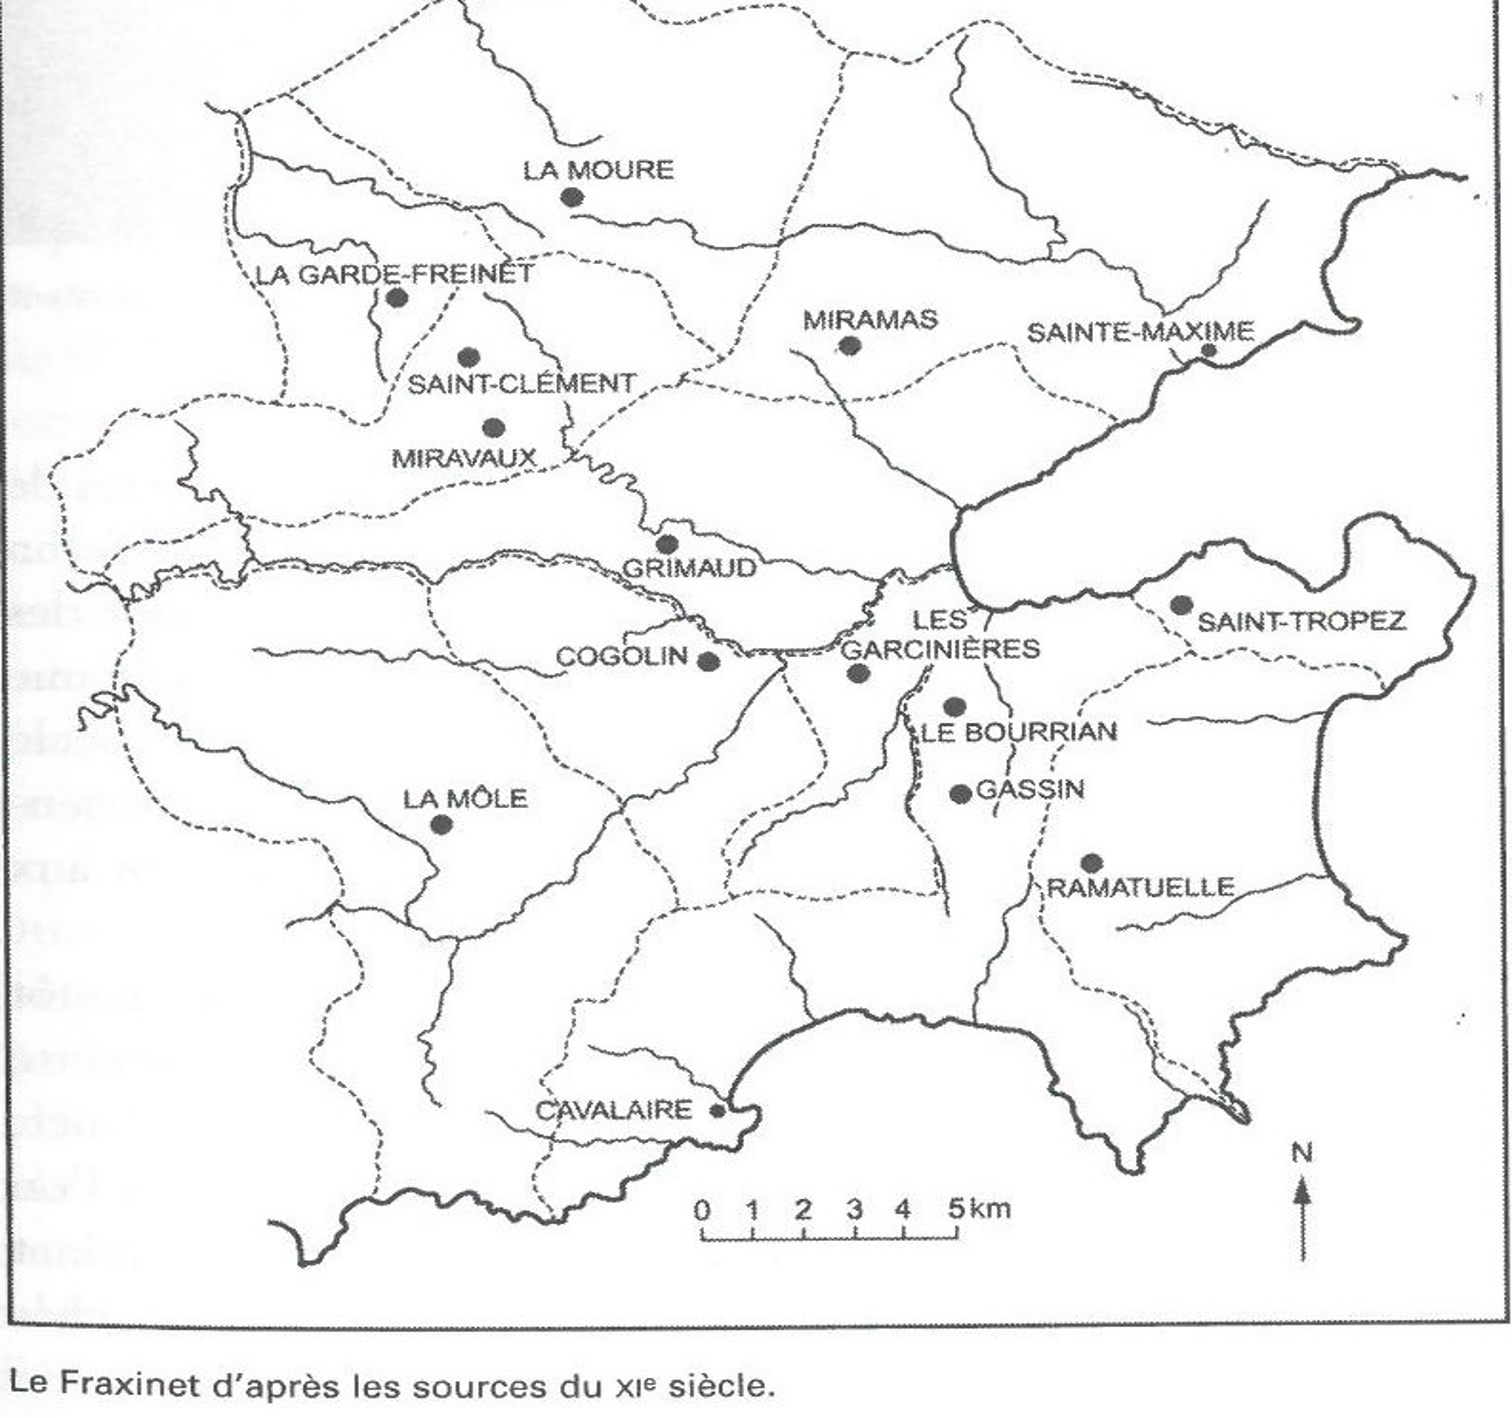
\includegraphics[width=\textwidth]{Images/Fraxinet.png}
    \caption{Le « Massif des maures » (Fraxinet) }
    \label{fig:Fraxinet}
\end{figure}

\paragraph{Des tombes musulmanes du début du Moyen-Âge à Nîmes (2016)}

3 sépultures à Nîmes avec une posture de corps du côté droit et le regard vers le sud est (direction de la Mecque). Un surcreusement pour placer le corps. Grâce à des analyses paleo-génétiques, des marqueurs du nord de l'Afrique.

\paragraph{Découverte récente (en Espagne)}

400 tombes découvertes dans la province de Saragosse orientées vers la Mecque, certainement des premières générations de musulmans installés dans la péninsule suite au débarquement de Tarik Ibn Zyad en 711. Probablement des \textit{convertis à l'islam, mais qui ont une culture traditionnellement romaine, donc ils apportent la preuve d'un moment de transition culturelle}.


\paragraph{Les Croisades, 1095-1291}
lancées par le pape Urbain II depuis Clermont.

\paragraph{1798: Expédition d’Egypte par Napoléon}
(essor de l’Orientalisme)

\paragraph{1830: tutelle coloniale sur l’Algérie qui durera 130 ans.}
Suivront l’Afrique de l’Ouest, le Maroc (« Protectorat »), la Tunisie, la Syrie-Liban.


\section{Sujets coloniaux, soldats, travailleurs, puis citoyens}

différentes qualifications de la présence musulmane en France.

\subsection{Participation de centaines de milliers de soldats nord-africains et ouest-africains aux deux guerres mondiales, au sein de l’armée française}

(se forme à cet occasion les premières bases d’une proto-aumônerie militaire musulmane)
\begin{figure}
    \centering
    \includegraphics[width=\textwidth]{Images/MosqueeFrejus.jpg}
    \caption{La Mosquée de Fréjus, édifiée en 1928 et de style malien, pour les tirailleurs sénégalais de Frejus}
    \label{fig:Frejus}
\end{figure}
\subsection{1905: fondation mosquée de St Denis de La Réunion}
(par des émigrés indiens du Gujarat)

\subsection{Accord dès 1767 signé entre Sidi Mohammed Ben Abdallah (Roi du Maroc) et Louis XV pour une première mosquée en France}
 mais qui ne verra pas le jour.


\subsection{1926: Grande mosquée de Paris}
début du crédit accordé puis des travaux en 1920

\paragraph{tentatives avortées en 1846}
le oomte de Pommereux, répond : 
\begin{quote}
« Il m'a
toujours paru difficile de pouvoir fonder une mosquée à Paris. Les
musulmans n'ont pas deux lois, mais une seule. Si ce n'était
qu'une loi religieuse, cela aurait peu d'inconvénients; mais c'est
en même temps une loi civile, opposée au principe même de notre
constitution, ce qui pourrait devenir pernicieux, parce que l' on ne
peut pas séparer l'une de l'autre. D'ailleurs, vous connaissez
l'esprit anti-progressif, intolérant du Koran. Et puis, écrit, rédigé
pour un peuple nomade, qui avait besoin de trouver sous sa main
la solution des questions civiles et religieuses, il ne convient plus
aussi bien à des populations stables. »
\end{quote}
La réaction du ministère de la Justice et des Cultes est~négative parce que les musulmans sont en faible nombre et ne l'ont pas demandé.

Un édifice au père lachaise est construit en 1857 pour le soins des défunts et leurs funérailles.

\paragraph{Un exemple de converti au XIXeme : Philippe Grenier}
Image d'un hoimme aux convictions sincères mais le caractère ostentatoire des prières en public.
\begin{figure}
    \centering
    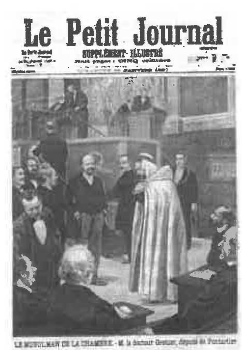
\includegraphics[width=\textwidth]{Images/DocteurGrenier.png}
    \caption{le docteur Grenier converti à l'islam à la chambre des députés, \textit{le Petit Journal}
24 Janvier 1817.}
    \label{fig:my_label}
\end{figure}

\paragraph{La société des Habous à la Mecque}
autre impulsion conduisant à la création de la Mosquée de
Paris est la mise en place, par le Quai d'Orsay, de la Société des
habous en 1916-1917. Celle-à est liée à la diplomatie de guerre
menée par la France au Proche-Orient. Pour contrer les menaces
sur les colonies à population musulmane que l'appel du calife au
\emph{jihâd} fait peser, la France a contracté une alliance avec le cherif
Hussein de la Mecque qui déclenche la révolte arabe contre les
Turcs dam le Hedjaz le 10 juin 1916. C'est la grande mission de
Si Kaddour Ben Ghabrit (186~-1954), un Algérien entré au service
de l'administration du protectorat au Maroc en 1892 et
agent diplomatique français de grande envergure.
Le chef du gouvernement Aristide Briand, envoie Ben Ghabrit à
la tête d'une délégation de pèlerins nord-africains après avoir
décidé la réouvertur du pèlerinage de La Mecque le 2 aout 1916.
Dans le but de péreniser la présence française, il est statué finalement
sur 1a question de l hôtellerie des pèlerins à la Mecque.
Celle-ci avait été évoquée en 1915 par la Commission interministerielle
des affaires musulmanes mais le gouvernement Général
de l'Algérie s'y était opposé. De la même manière il s'oppose
au projet de « Village kabyle » comprenant notamment une mosquée.
envisagé par la chambre de commerce de Marseille en
1917. Mais le Parlement vote un crédit de 500000 francs le
31 janvièr 1916 et Pierre de Margerie (1861-1942), ancien secrétaire
général de la conférence d'Algesiras pour le Maroc (1906)
et directeur des Affaires politiques au Quai d'Orsay pendant toute
la guerre, organise le dispositif exécutoire qui débouche sur
l'achat d'un batiment à La Mecque et la création de 1a Société des
babous comme organisme propriétaire et administrateur.
Seul-un bien habous, en effet, c'est-à-dire une propriété de type
religieux inalienable, insaisissable et imprescriptible, autorisait
la détention indirecte par le gouvernement français d'un bien
immobilier dans l'enceinte de La Mecque. Et un tel bien habous
devait être administré par une Société des babous (on dirait
aujomd'hui une association). C'est Pierre de Margerie qui en
désigne lui-même les membres, parmi lesquels Si Kaddour Ben
Ghabrit qu'il charge de la presidence de la comission chargée de la création. 

\begin{Synthesis}
On voit comment
s'imbriquent le devoir religieux qui incombe à la France en tant
que puissance musulmane et les impératifs diplomatiques.
Cette société des Habous est encore propriétaire des lieux de la Mosquée de Paris
\end{Synthesis}

\paragraph{Loi française et inspiration marocaine : l'institut musulman}
Edouard Herriot, partie radical, à la suite de l'effort de guerre de la main d'oeuvre venus des colonie, a un respect de libre penseur pour l'Islam : "Encourageons cet islam qui s'éveille ou se réveille". En 1920, il fait voté 500 000 francs pour la mosquée de Paris "vraie maison de l'Islam".

Il est étonnant de noter qu'après la loi de séparation de l'Eglise et l'Etat, une telle subvention ait pu être votée. Un sénateur, Dominique Delahaye, note : "puisqu'on parle des musulmans, il serait bientôt temps de traiter les catholiques aussi bien que les musulmans".

L'architecte choisi est Maurice Tranchant de Lunel, appartenant à l'entourage Lyautéen de Rabat et qui a beaucoup voyagé. La mosquée s'inspire de l'architecture marocaine, mais aussi de l'Espagne d'al Andalus et de l'Inde musulmane. 

A leurs côtés,
Maurice Co1rat représente le gouvernement. Il est l'auteur de
1a fameuse formule, attribuée parfois à tort à Lyautey :
\begin{quote}
    « Quand
il s' érigera, au-dessus des toits de la ville, le minaret que vous
allez construire à cette place, il ne montera vers le beau ciel
nuancé de l'Île-de-France qu'une prière de plus, dont les tours
catholiques de Notre-Dame ne seront point jalouses. »
\end{quote}

L'inauguration de la Mosquée de Paris a lieu le 15 juillet 1926 en présence du président Gaston Doumergue et du sultan du Maroc. Le discours de Si Kaddour Ben Ghabrit 
\begin{quote}
    
Ma confusion le dispute à
ma fierté de voir ici réunis le plus haut représentant de la nation
~ et Sa Majesté le sultan Maroc. Cette réunion est symbo1ique. Elle marque que 1a France, fidèle à une politique plusieurs
fois sécu1aire affirme d'éclatante manière la sympathie qu'elle ressent pour les musulmans de toutesorigines qui sont pour elle également des amis. Cet homage de haut et noble libéralisme aura, a déjà eu le plus grand retenstissement dans le monde musulman car il démontre que la France hospitalière à toutes les races ne l'est pas moins à toutes les idées, à toutes les religions. \end{quote}

Gaston Doumergue n'hésite pas à citer un \emph{hadith} du Prophète consistant à définir le meilleur islam : 
\begin{quote}
    c'est celui du croyant dont les musulmans n'ont à redouter ni la main ni la langue
\end{quote}
et à conclure : "cet islam-là est aussi le notre".


il y eu des réactions comme Charles Maurras : 
\begin{quote}
    Cette mosquée en plein Paris ne me dit rien de
bon. Il n'y a peut être pas de réveil de l'islam, auquel cas tout ce
que je dis ne tient pas et tout ce que l'on fait se trouve être la plus vaine des choses. Mais, s'il y a un réveil de l'islam, et je ne
crois pu que l'on en puisse en douter, un trophée de la foi coranique sur cette colline Sainte-Geneviève où tous les plus grands docteurs
de la chrétienté enseignèrent contre l'islam ~ plus
qu'une offense à notre passé : une menace pour notre avenir. 
\end{quote}



\subsection{Le projet Blum Viollette}
Le projet de loi relatif à l'exercice des droits politiques par certaines catégories de sujets français en Algérie, dit le projet Blum-Viollette (1936), fut un projet de loi du Front populaire de Léon Blum, sur les propositions de Maurice Viollette, ancien gouverneur général d'Algérie, visant à ce que 20 000 à 25 000 musulmans puissent devenir citoyens français tout en gardant leur statut personnel lié à la religion. Le projet, délibéré en Conseil des ministres le 15 octobre 1936, est déposé sur le bureau de la Chambre des députés le 30 décembre suivant. La commission du suffrage universel l'éxamine en 1938, mais celui-ci est définitivement suspendu le 4 mars.


\section{Evolution de la présence musulmane en France (chiffres, nombre de lieux de
culte…)}

\paragraph{Immigration de travail}
- à partir des années 50, a fortiori après loi regroupement familial (décret d’avril 1976, étendu par un arrêt du CE de 1978)
-200.000 « nord-africains » en 39, 1.600.000 « musulmans » tout pays d’origine confondus en 1985 (Krieger, 1985), 3,65 millions dont moitié de nationalité fra. (INED-INSEE, 2004), 4 à 5 millions de français de confession musulmane de nos jours.

\paragraph{Lieux de Cultes}
 (approx.); autour de 100 en 1970, de 500 en 1985, de 1300 en 1992, de 1600 en 2003, de 2500 en 2014, autour de 3000 de nos jours (France et TOM).

\paragraph{de sujets à citoyens}
-Sadek SELLAM (voir biblio) parle d’un passage de « sujets » (1830-1947) à « citoyens » (1947-2004).


\section{Bibliographie de la partie}
ARKOUN Mohammed (dir.), Histoire de l’islam et des musulmans en France, Albin
Michel, 2006.
KRIEGER-KRYNICKI Annie, Les musulmans en France, Maisonneuve et Larose,
1985.
SELLAM Seddak, La France et ses musulmans, Fayard, 2006.
-Support multimédia :
Documentaire « Nous, Français musulmans », Arte, Janvier 2020, 2 parties X 52’ :
https://www.arte.tv/fr/videos/084758-001-A/nous-francais-musulmans-1-2/ et
https://www.arte.tv/fr/videos/084758-002-A/nous-francais-musulmans-2-2/
Emission « L’islam et la République » (52’), de Questions d’islam, France culture,
pres. Ghaleb Bencheikh, invité Haouès Seniguer (Mcf Univ. Lyon);
https://www.franceculture.fr/emissions/questions-dislam/lislam-et-la-republique